%%%%%%%%%%%%%%%%
%%  Template for latex documents
%%  Author: Marco A. Aquino-Lopez
%%  Nota: to get a word document use pandoc
%%  pandoc -f latex Articulo.tex -o Articulo.docx --bibliography=bibliography.bib
%%%%%%%%%%%%%%%%%
%\documentclass [twocolumn,10pt] {article}
\documentclass [10pt] {article}
\usepackage [utf8] {inputenc}
\usepackage[english]{babel}

\usepackage {graphicx}
\usepackage {amsfonts}
\usepackage {amsthm}
\usepackage {amsmath}
\usepackage {natbib}
\usepackage[in]{fullpage} %To have more in the page
%.____         ___________    ____  ___ 
%|    |   _____\__    _______ \   \/  / 
%|    |   \__  \ |    |_/ __ \ \     /  
%|    |___ / __ \|    |\  ___/ /     \  
%|_______ (____  |____| \___  /___/\  \ 
%        \/    \/           \/      \_/ 

\graphicspath{{Figures/}} %Setting the graphicspath

%Extra packages
\usepackage{placeins}

%%%%%%

\date{ }
\usepackage{color}

%%%% To mark notes or added text by Author1 (a1)
%%%% This allows to add notes
%\newcommand{\a1}{\color{red} }  %% begin
%\newcommand{\1a}{ \color{black}} %% end
%\newcommand{\cuta1}[1]{\ac [cut] \ca} %% to mark cut text
%\newcommand{\notea1}[1]{\textcolor{red}{(note)}\footnote{\ac #1 \ca}}  %% To add a note or comment


%%%% To mark notes or added text by Andres (ac)
\newcommand{\ac}{\color{red} }  %% begin
\newcommand{\ca}{\color{black}} %% end
\newcommand{\cutac}[1]{\ac [cut] \ca} %% to mark cut text
\newcommand{\noteac}[1]{\textcolor{red}{(note)}\footnote{\ac #1 \ca}}  %% To add a note or comment

%%%% To mark notes or added text by Andres (ac)
\newcommand{\ma}{\color{blue} }  %% begin
\newcommand{\am}{\color{black}} %% end
\newcommand{\cutma}[1]{\ac [cut] \ca} %% to mark cut text
\newcommand{\noteam}[1]{\textcolor{red}{(note)}\footnote{\ac #1 \ca}}  %% To add a note or comment


% NOTE: To produce blinded version, replace "0" with "1" below.
\newcommand{\blind}{1}
\newcommand{\papertitle}{
\ac A simulation study to compare $^{210}$Pb dating data analyses \ca}

\begin{document}
	\def\spacingset#1{\renewcommand{\baselinestretch}%
		{#1}\small\normalsize} \spacingset{1}
	%%%%%%%%%%%%%%%%%%%%%%%%%%%%%%%%%%%%%%%%%%%%%%%%%%%%%%%%%%%%%%%%%%%%%%%%%%%%%%
	\if1\blind
	{
		\title{\textbf{\papertitle}}

		\author{Marco A Aquino-L\'opez\thanks{
				Centro de Investigaci\'on en Matem\'aticas (CIMAT),
				Jalisco s/n, Valenciana, 36023 Guanajuato, Gto, Mexico.
				email: \texttt{aquino@cimat.mx} } \thanks{Corresponding author.}
					\and
			Nicole K. Sanderson\thanks{
				GEOTOP Research Centre, Universit\'e du Qu\'ebec \'a Montr\'eal, 
				Montr\'eal, Qu\'ebec, H2X 3Y7, Canada. 
				email: \texttt{sanderson.nicole@uqam.ca}}
					\and
			Maarten Blaauw\thanks{School of Natural and Built Environment,
				Queen's University Belfast,
				Belfast, BT7-1NN, UK.
				email:\texttt{maarten.blaauw@qub.ac.uk}  }
					\and
			J Andr\'es Christen\thanks{
				Centro de Investigaci\'on en Matem\'aticas (CIMAT),
				Jalisco s/n, Valenciana, 36023 Guanajuato, Gto, Mexico.
				email: \texttt{jac@cimat.mx}  }
			}
		\maketitle
	} \fi

	\if0\blind
	{
		\bigskip
		\bigskip
		\bigskip
		\begin{center}
			{\LARGE\bf \papertitle}
		\end{center}
		\medskip/
	} \fi

	\bigskip
\begin{abstract}
    The increasing interest in understanding the impact of humans have on the environment, has lead to a considerable number of studies focusing on the analysis of sediment accumulation for the last 200 years. 
Dating this period is often complicated by poor chronological resolution and large errors associated with recent radiocarbon (14C) ages, which is the most popular dating technique. 
The use of lead-210 ($^{210}$Pb) is a popular method as it allows for the measurement of absolute and continuous dates for this period of time.
$^{210}$Pb dating method has traditionally relied on the Constant Rate of Supply (CRS) model which uses the radioactive decay equation resulting in a restrictive model to approximate dates.

    Recent studies in radiocarbon age-depth models \citep{Blaauw2018} have shown that the Bayesian age-depth models provide a more reliable and trustworthy chronology.
Following the recent development of \textit{Plum} \citep{Aquino2018}, the only Bayesian alternative to $^{210}$Pb dating model, this work presents a thorough and objective comparison between the classical approach to $^{210}$Pb dating (CRS) and its Bayesian alternative (\textit{Plum}).
	Three different simulations, representing three different sedimentation processes and meeting the assumptions imposed by the CRS model, were used to produce a fair and honest comparison.
Results from this study not only confirms the results obtained by \citet{Blaauw2018}, they also show a series of worrying outcomes regarding the accuracy and precision of the CRS model, mainly that the uncertainty associated with the model is consistently insufficient to capture the true values even when the sediment is entirely dated.
In addition, the CRS model does not appear to improve its accuracy as more information is available, which results in a model for which accuracy is chaotic and unpredictable.
On the other hand, the Bayesian alternative (\textit{Plum}) provides consistently accurate results even with few samples, and its accuracy and precision constantly improve as more information is available.
\end{abstract}
	\noindent%
	{\it Keywords:} Plum, Age-depth models, Chronology, Constant Rate of Supply, Comparison.
	\vfill
	\newpage
	\spacingset{1.45} % DON'T change the spacing!

%%%%%%%%%%%%%%%%%%%%%%%%%%%%%%%%%%%%%%%%%%%%%%%%%%%%%%%%%%%%%
%%%%%%%%%%%%%%%%%%%%%%%%%%%%%%%%%%%%%%%%%%%%%%%%%%%%%%%%%%%%%
\section{Introduction}

Lead-210 ($^{210}$Pb) is a radioactive nuclide,part of the $^{238}$U decay chain, which forms naturally in the atmosphere as well as in sediments.
This isotope, with a half-life of 22.23 years, is commonly used to date recent recently accumulated sediments ($<150$ to $200$ years). 
Unlike to other dating techniques such as $^{14}$C (radiocarbon dating), using a single measurement of $^{210}$Pb is not possible for dating; it is only when a suitable portion of the decay curve (the total inventory) is measured and with certain assumptions about the sedimentation process are met that a chronology can be established.  
In recent decades, increasing amounts of palaeoecological and pollution studies have focused on recent sediments \citep[e.g.,][]{Courtney2019} in order to evaluate human impacts on the environment.
These studies strongly rely on the accuracy of their chronologies in order to correctly assign dates to chemical, biological and ecological changes.
That is, unlike other dating techniques, an analysis of a series (data set) of $^{210}$Pb measurements most be carried out in order to obtain meaningful dates.  In a lake sediment, or any other, sedimentation process, samples are taken along a core at different depths, from which $^{210}$Pb activity is measured.  
The whole series of $^{210}$Pb measurements need to be analyzed to attempt to produce a coherent chronology, see \cite{Aquino2018}.

A range of traditional data analyses, or so called ``models'', are available for dating recent sediment using $^{210}$Pb, most notably are the Constant Rate of Supply (CRS), Constant Flux:Constant sedimentation (CF:CS) and Constant Initial Concentration (CIC) models \citep{Appleby1978,Robbins1978,Sanchez-Cabeza2012} . 
The CRS model, also known as Constant Flux - (CF) model is by far the most popular (see Figure \ref{fig:210models}) and has the most flexible assumptions. 
The CRS model assumes a constant supply of $^{210}$Pb to the sediment from the atmosphere and allows for changes in the sedimentation rate. 
In order to build a chronology, the CRS model uses a ratio between the complete ``inventory'' (the complete estimate of the radioactivity in the sediment column of the sediment between the surface and the ``equilibrium depth'' where $^{210}$Pb from the atmosphere can no longer be found) and the remaining  inventory from depth $x$ ($t(x)=\frac{1}{\lambda}\log\left( \frac{A_0}{A_x}\right)$, where $A_0$ is the complete inventory and $\lambda$ the decay constant of the $^{210}$Pb $\approx .03114$).

Other, more restrictive models such as CF:CS and CIC requiere the assumption of a constant supply of $^{210}$Pb as well as other assumptions of the sedimentation process, as well as that of a constant supply of $^{210}$Pb.
The flexibility of the CRS, regarding its assumptions, comes at the cost of the need to measure a sufficient portion of the inventory or the use of interpolation in order to properly estimate the complete inventory of $^{210}$Pb in the sediment. 

The CRS model has undergone several revisions in the last decade in order to improve its accuracy and applicability. 
There are two types of revisions to this model: (1) revisions to its uncertainty estimates \citep{Binford1990,Appleby2001,Sanchez-Cabeza2014} and (2) to its application where extra information is available, such as external independent dating markers (e.g. $^{137}$Cs dates) or laminated sediments \citep{Appleby1998,Appleby2001,Appleby2008}.

A recent inter-laboratory model comparison experiment \citep{Barsanti2020} presented concerning results.
A series of $^{210}$Pb measurements were send to 14 laboratories around the world.
Each laboratory was ask to provide a chronology, given the same data.
This experiment resulted in a wide range of chronologies not only when different models were used, but even when the same model was applied.
The authors strongly recommended to the use of independent time markers (independent dating sources) to validate of the chronologies.
This research clearly and critically shows the impact that user decisions have on the resulting chronologies, which becomes extremely important when trying to replicate and/or update the resulting chronologies.
Users attending to do so will not only need access to the raw data but also to every user decision in constructing the chronology; unfortunately, these raw data sets and decisions are rarely reported.


\begin{figure}[h!]
	\begin{centering}
		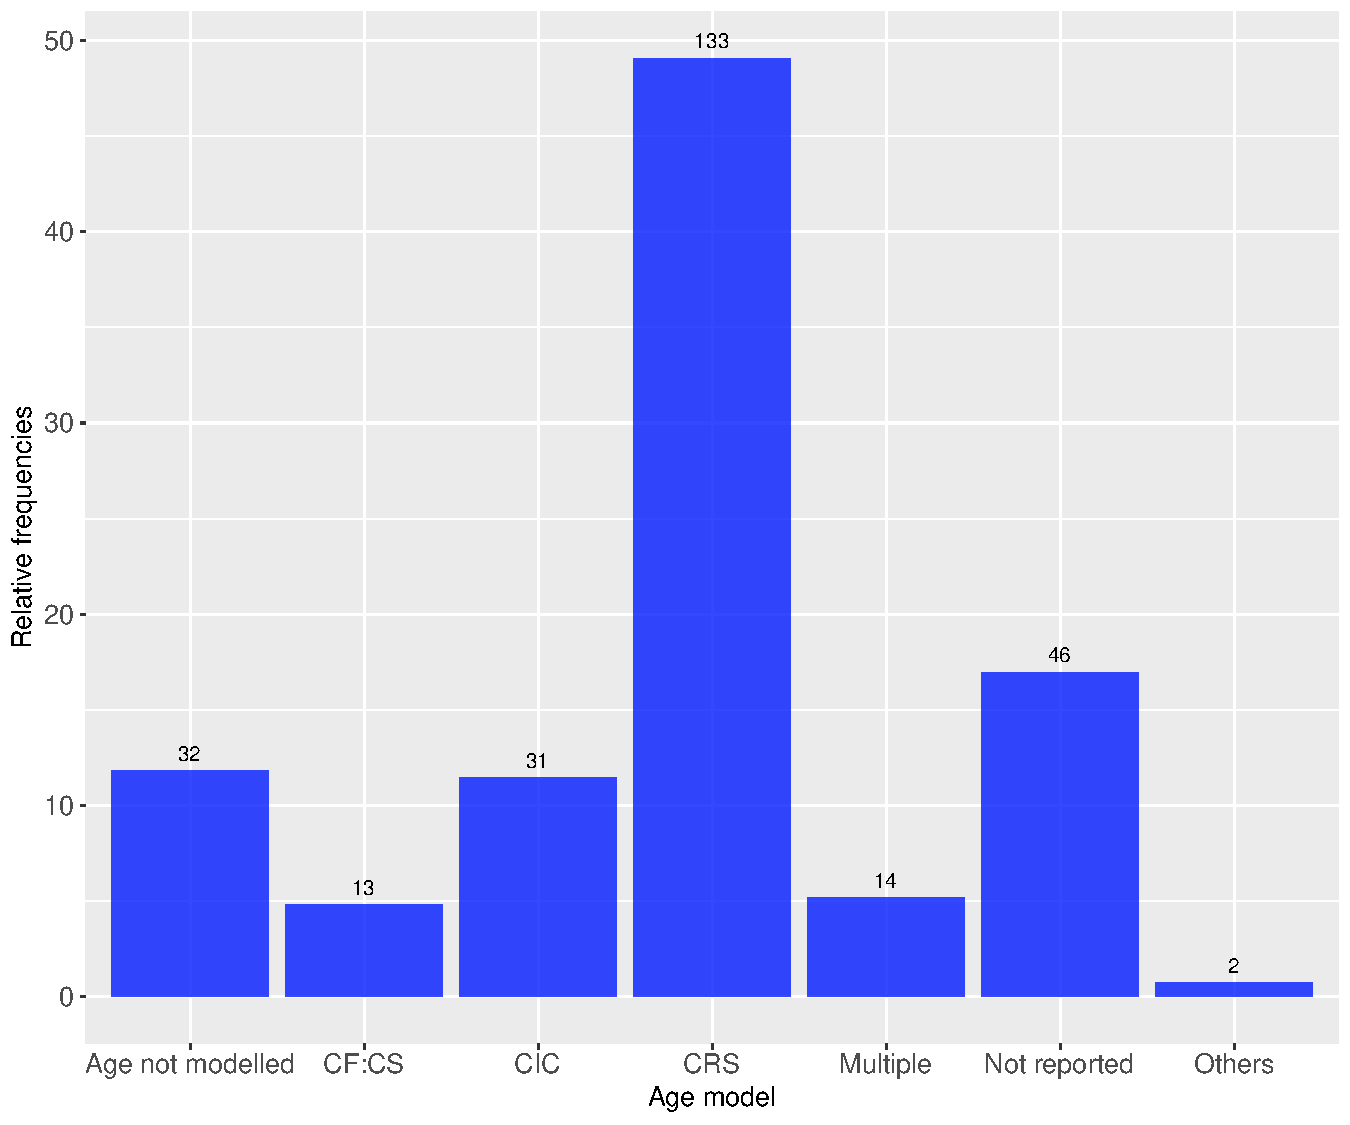
\includegraphics[width=.75\linewidth]{210Pbmodels-bar.pdf}
		\caption{Frequency of $^{210}$Pb dating models used in papers between 1964 and 2017. Data gathered by \citet{Courtney2019} from a literature review of 271 papers. The models include CF:CS model \citep[The Constant Flux - Constant Sedimentation;][]{Robbins1978}, CIC (Constant Initial Concentration) \citep{Goldberg1963,Crozaz1964,Robbins1978} and CRS -  \citep[Constant Rate of Supply;][]{Appleby1978,Robbins1978}. }
		\label{fig:210models}
	\end{centering}
\end{figure}

Recently \citet{Aquino2018} presented an alternative to these classical models, by introducing \textit{Plum}, a Bayesian approach to $^{210}$Pb dating.
This model treats every data point as originating from a system that includes the sedimentation process as well as the radioactive decay process. 
It also incorporates an important variable to the inferred processes, namely, the levels of supported $^{210}$Pb, which naturally forms in the sediment and is normally threaded as a hindrance variable.
\textit{Plum} assumes that there exists an (unknown) age-depth function $t(x)$ that relates depth $x$ with calendar age $t(x)$.  Conditional on $t(x)$, the following model is assumed for measured $^{210}$Pb $y_i$ for the sediment section form depths $x_i - \delta$ to $x_i$
\begin{eqnarray}
y_i\mid P^S_i, \Phi_i, \bar{t}\sim \mathcal{N} \left(A^S_i+\frac{\Phi_i}{\lambda} \left( e^{-\lambda t(x_i-\delta)} - e^{-\lambda t(x_i)} \right), (\sigma_i\rho_i)^2 \right). 
\end{eqnarray}
Here $y_i$ is the total amount of $^{210}$Pb in a sample, $A_i^S$ is the supported $^{210}$Pb in the sample and $\Phi_i$ the supply of $^{210}$Pb to the sediment, see \cite{Aquino2018} for details. 
The age-depth model $t(x)$ is based on a piece-wise linear model constrained by prior information on the sediment's accumulation rates  \citep{Blaauw2011}.%and its variability

This treatment of the data allows for a formal statistical inference and by using a Bayesian approach all the parameters of the model can be inferred.
This differs from the CRS model as the latter uses the decay equation to obtained the age-depth function resulting in a more restrictive age-depth model, removes assumed values of supported $^{210}$Pb before modelling, and does not provide a formal statistical inference.
\textit{Plum} has shown to provide accurate results with a realistic precision depending on the different case scenarios \citep{Aquino2020} - both in simulations as well as for real cores.
Under optimal conditions \textit{Plum} and the CRS model have shown to provide similar results \citep{Aquino2020} with \textit{Plum} providing more realistic uncertainties, with minimal user interaction. 

\citet{Blaauw2018} presented a comparison between classical and Bayesian age-depth models construction, both for real and simulated $^{14}$C-dated cores.
They concluded that Bayesian age-depth models provide a more accurate result and more realistic uncertainties under a wide range of scenarios.  
Similarly, \textit{Plum} has shown to provide accurate results with a realistic precision depending on different scenarios, both in simulations as well as for real cores. Under optimal conditions, \textit{Plum} and the CRS model have shown to provide similar dates , with \textit{Plum} providing more realistic uncertainties with minimal user interaction. 
In this study, we compare $^{210}$Pb dates and uncertainties from the widely applied CRS model (by far the most popular age-depth model for $^{210}$Pb) against \textit{Plum} using simulated cores, i.e. sedimentation ``scenarios''.
The objective of this study is to test whether the results obtained by \citet{Blaauw2018}, concerning the accuracy and precision of the Bayesian approach, are maintained in a more complex modelling situation, such as the construction of $^{210}$Pb-based age-depth models.
We also wish to observe the learning process of each of the models and estimate the amount of information is needed to obtained a reasonable chronology for each model. 

The paper is organized as follows: first section sets the tools for the comparison, it describes the simulations of the three different scenarios and we described a parameter which will facilitate the comparison called information percentage. 
Section 3 describes the comparison for both the overall chronologies and by single depths.
Lastly section 4 presents the conclusions and discussion of the results obtained in section 3. 



%%%%%%%%%%%%%%%%%%%%%%%%%%%%%%%%%%%%%%%%%%%%%%
%%%%%%%%%%%%%%%%%%%%%%%%%%%%%%%%%%%%%%%%%%%%%%
\section{Experiment Setup: Simulations}

	In order to observe the accuracy and precision of any model, a known true age-depth function is required.
\citet{Blaauw2018} presented a methodology for simulating radiocarbon dates and their uncertainties, while \citet{Aquino2018} presented an approach for simulating $^{210}$Pb data given an age-depth function $t(x)$.
It is important to note that these simulations follow the equations presented by \cite{Appleby1978, Robbins1978} guaranteeing that the CRS assumptions are met. 
By using the approach presented by \citet{Aquino2018} for simulating $^{210}$Pb data and the structure of uncertainty estimation presented by \citet{Blaauw2018}, reliable $^{210}$Pb simulated data can be obtained.

\subsection{Simulation Construction}\label{sec:SimConst}

Three different scenarios (see Table \ref{tab:sim_param}) were chosen for our sedimentation simulations, each with their own age-depth functions and parameters. 
These scenarios were selected as they provide three key challenges for the models: Scenario 1 presents an age-depth function which is quite common for recent sediments, with less compaction toward the surface at 0 cm depth; Scenario 2 presents a challenging core structure as the function replicates a drastic and rapid shift in sediment accumulation behaviour around depth 15 cm depth; and lastly Scenario 3 presents a cyclic and periodic change in accumulation rates. 
Using the age-depth functions and defined parameters defined in Table \ref{tab:sim_param}, we obtain the $^{210}$Pb activity, or concentration, at any given depth or interval by integrating the age-depth curve for that interval.  
These concentrations may be interpreted as error-free measurements, 
see Figure \ref{fig:true_210} . 
Because $^{210}$Pb activity measurement is subject to error, we need to replicate the measurement errors. 
\citet{Blaauw2018} presents error structure for radiocarbon dates. 
We can use this structure to our $^{210}$Pb measurements as both measurements are subject to similar measurement problems. 


\begin{table}[!h]
	\centering
	\begin{tabular}{l|ccc}
Label    	& 	Age-depth		&	$ \Phi$		& Supported $^{210}$Pb  \\
		&	function $t(x)$		&	($\frac{Bq}{m^2yr }$)	& ($\frac{Bq}{kg}$) 	\\ \hline
Scenario 1 	&	$\frac{x^2}{4} + \frac{x}{2}$	&	100	& 10	\\
Scenario 2 	&	$12x -.2x^2$			&	50	& 25	\\
Scenario 3 	&	$8x+25\sin(\frac{x}{\pi})$	&	500 	& 15		
	\end{tabular}
	\label{tab:sim_param}
	\caption{Simulated age-depth function and parameters used in each scenario}
 \end{table}

\begin{figure}[!h]
 \centering
  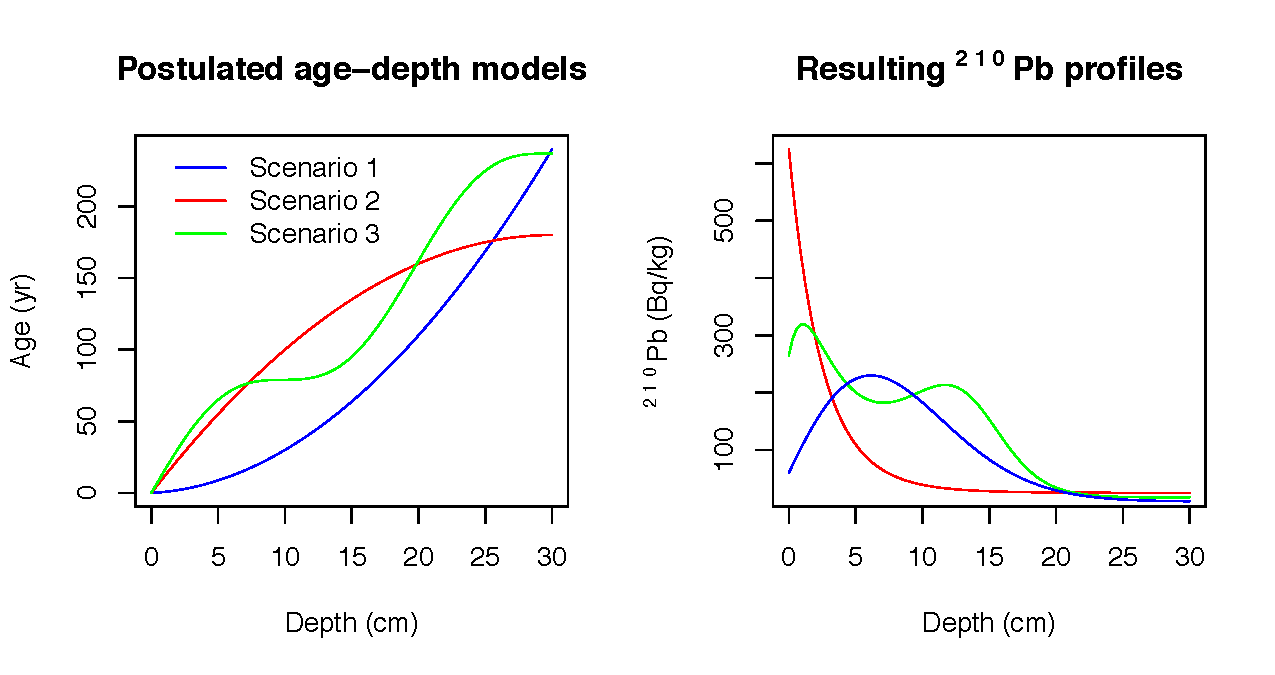
\includegraphics[width=.95\linewidth]{chronology.pdf}
	\caption{Simulated sedimentation scenarios with their corresponding $^{210}$Pb profiles. Left: Age-depth functions for the three different scenarios (Table \ref{tab:sim_param}). Right: Corresponding $^{210}$Pb activity profiles in relation to depth.}
  \label{fig:true_210}
\end{figure}


	Let $C_{\hat{x}}$ be the true  $^{210}$Pb concentration in the interval $\hat{x}=[ x-\delta, x)$, given the age-depth function $t(x)$ and parameters $\Phi$ and $A^S$ in each scenario. 
To simulate disturbances in the material, we can introduce scatter centred around the true value, $\theta \sim \mathcal{N}\left(C_{\hat{x}},y^2_{scat}\right)$, where $x^2_{scat}$ is the amount of scatter for this variable (in this case $y^2_{scat}=10$). 
Now, to replicate outliers, a shift from the true value ($x_{shift}$) is defined, which occurs with a probability $p_{out}$. This results in a new variable $\theta'$ which is defined as
\begin{align}
	\theta' = \begin{cases}
			\mathcal{U}(\theta - x_{shift},\theta + x_{shift}), &  p_{out} \\
			\theta, & 1-p_{out}
		\end{cases}.
\end{align}

	Finally, to simulate the uncertainty provided by the laboratory, we can define the simulated measurements as  $y(\theta')\sim\mathcal{N}\left(\theta',\sigma_R^2\right)$, where $\sigma_R$ is the standard deviation reported by the laboratory. 
$\sigma_R$ is defined as $\sigma_R= \max \left(\sigma_{min}, \mu(\theta')~\varepsilon~y_{scat}~\right)$, where $\sigma_{min}$ is the minimum standard deviation assigned to a measurement. This variable differs between laboratories,we use a default value of $1~ Bq/kg$. 
Finally, $\varepsilon$ is the analytical uncertainty (default .01) and $y_{scat}$ an error multiplier (default 1.5).
The default parameters were set in accordance with \citet{Blaauw2018}.

For this this study we created a data set for each of the three simulation by integrating in intervals of $\delta =$1 cm, for depths from  0 to 30 cm where radioactive equilibrium was guaranteed \citep{Aquino2018}.
The complete simulated $^{210}$Pb data sets can be found in the Supplementary Material \ref{sec:supp_mat}.



%\ac (where equilibrium was guaranteed) -- \ma esto si es importante paleoecologos \ac y es algo en lo que no debemos entrar en detalle pero >de donde salen estos parametros 1, 0.1, 1.5 etc ... explica o pon cita ... > see \citet{Blaauw2018} for details ?\ac.

%%%% Esto esta repetido al inico de la siguiente seccion y mucho mejor explicado
%\subsection{Percentage of information}

%	With these data sets, we then define a new variable called ``percentage of information''. This variable relates to how much of the available information was measured. 
%We assumed that background was reached at depth $m$, information percentage is define as how much area of the core was measured, e.g. if background \ac (no hemos explicado que es esto) background activity (where data $y_i$ is below a threshold $y_b$ ... si dices background activity es más claro a lo que te refieres)\ca was reached at depth $m=100$ cm and the core was sampled using 20 $1$ cm thick slices, the percentage of information would be 20 \%. This variable will help us to have a measuring tool for how much information is needed for a good chronology without depending on the number or size of the samples. 

%In order to compare both the CRS and \textit{Plum} models under simular circumstances, the previously described data sets will be randomly selected for samples given an information percentage. 
%In the case of cores which have not reached background, \textit{Plum} \citep{Aquino2018} has shown to provide accurate results without the need for user interference. 
%On the other hand, in such cases the CRS can only provide a chronology if the complete inventory is estimated using extrapolation and if the model is forced to pass through a known date (e.g., as estimated by a 137Cs peak related to the AD 1986 Chernobyl accident). .
%This means user intervention and to avoid this problem and to provide a more objective comparison, here every simulated sampling set will reach background, which guarantees the proper use of the CRS model. 

%%%%%%%%%%%%%%%%%%%%%%%%%%%%%%%%%%%%%%%%%%
%%%%%%%%%%%%%%%%%%%%%%%%%%%%%%%%%%%%%%%%%%
\section{Model Comparison}

To allow for a reasonable comparison between models, and to evaluate the effect that different percentages of information may have on the accuracy and precision of $^{210}$Pb models, we used our three simulated data sets (see previous section). 
For these simulated cores, samples were randomly selected given a percentage of information (e.g. for a 20\% information data set, 6 random 1-cm samples were selected of a possible total 30 1-cm samples). 
As the CRS model assumes that background has been reached, in order to reduce user manipulation, we decided to fix the last sample (30 cm depth) for every case.
This step not only guarantees the consistent application the CRS model, it also provides the model with single bottom-most depth to be removed as it is common practice when using the CRS model.
100 different samples were randomly selected for information percentages from 10\% to 95\% at 5\% intervals (i.e., 10\%, 15\%, 20\%,...,95\%) and the complete sample was also used (i.e 100\% percentage of information sample).
After a random sample was selected, both the CRS model and \textit{Plum} were applied to the data set.  
To have an objective comparison, both models were run with their default configuration (\textit{Plum} with default settings and CRS estimates and uncertainties as described in \citet{Appleby2001}). 
Both sets of outputs were then compared against the true known age value.

\begin{figure}[!]
	\begin{centering}
		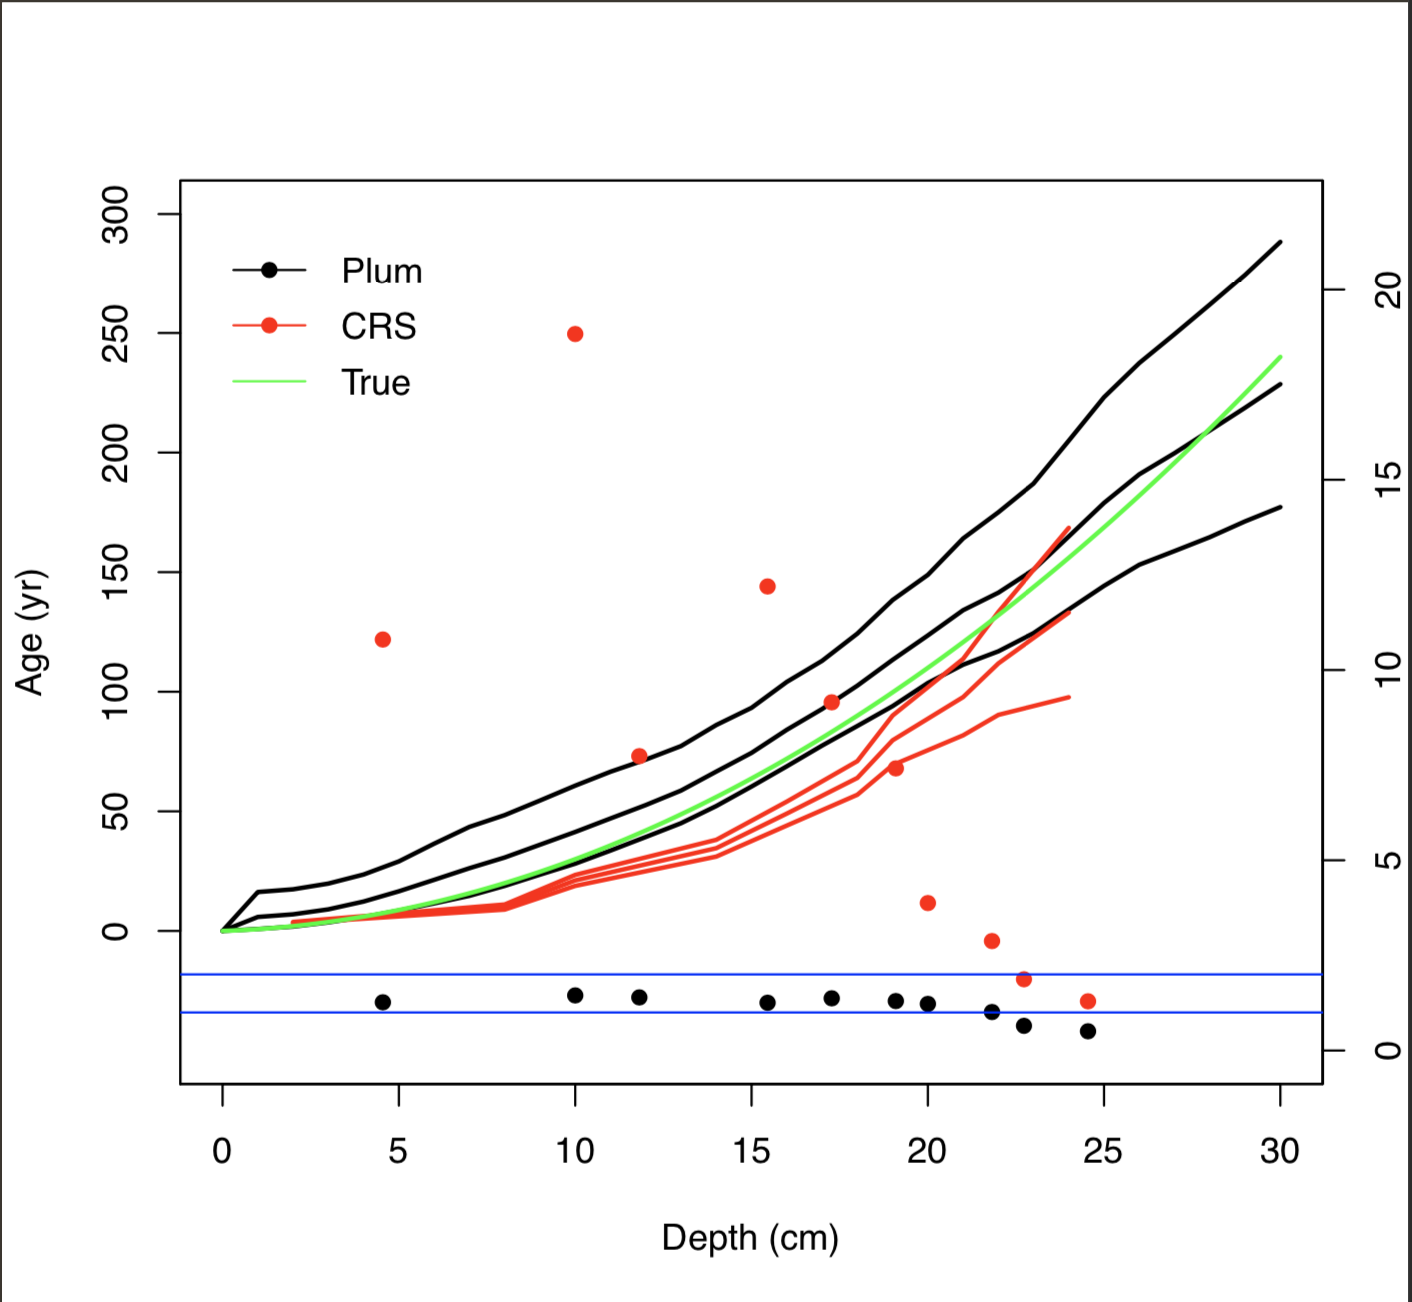
\includegraphics[width=\linewidth]{comparison1.png}
		\caption{Comparison between \textit{Plum} and the CRS model against the true age-depth model using 50\% of the information percentage (using 1-cm samples at depths 2, 8, 10, 14, 16, 18, 19, 21, 22, 24, 25, 27, 28, 29, 30). Lines show the age estimates with the 95\% credible intervals (\textit{Plum}) and the 95\% confidence interval (CRS). Dots show the normalized offset, distance between the inferred age and the true age in relation to the standard error (the standard deviation in the case of the CRS and the length of the confidence interval divided by 4 in the case of \textit{Plum}).    }
		\label{fig:comparison1r}
	\end{centering}
\end{figure}

Figure \ref{fig:comparison1r} shows an example of the comparison between the $^{210}$Pb models against the true value. 
As we are dealing with a total of $n =$ 5333 simulations, in order to evaluate the overall precision and accuracy of bothmodels, we decided to calculate the mean offset to the true age-depth model (in yr), the mean of length of the 95\% intervals (in yr), as well as the mean normalized accuracy indicating the distance of modelled ages from the true value given the model's own uncertainty at each depth.  

\begin{figure}[!]
 \centering
  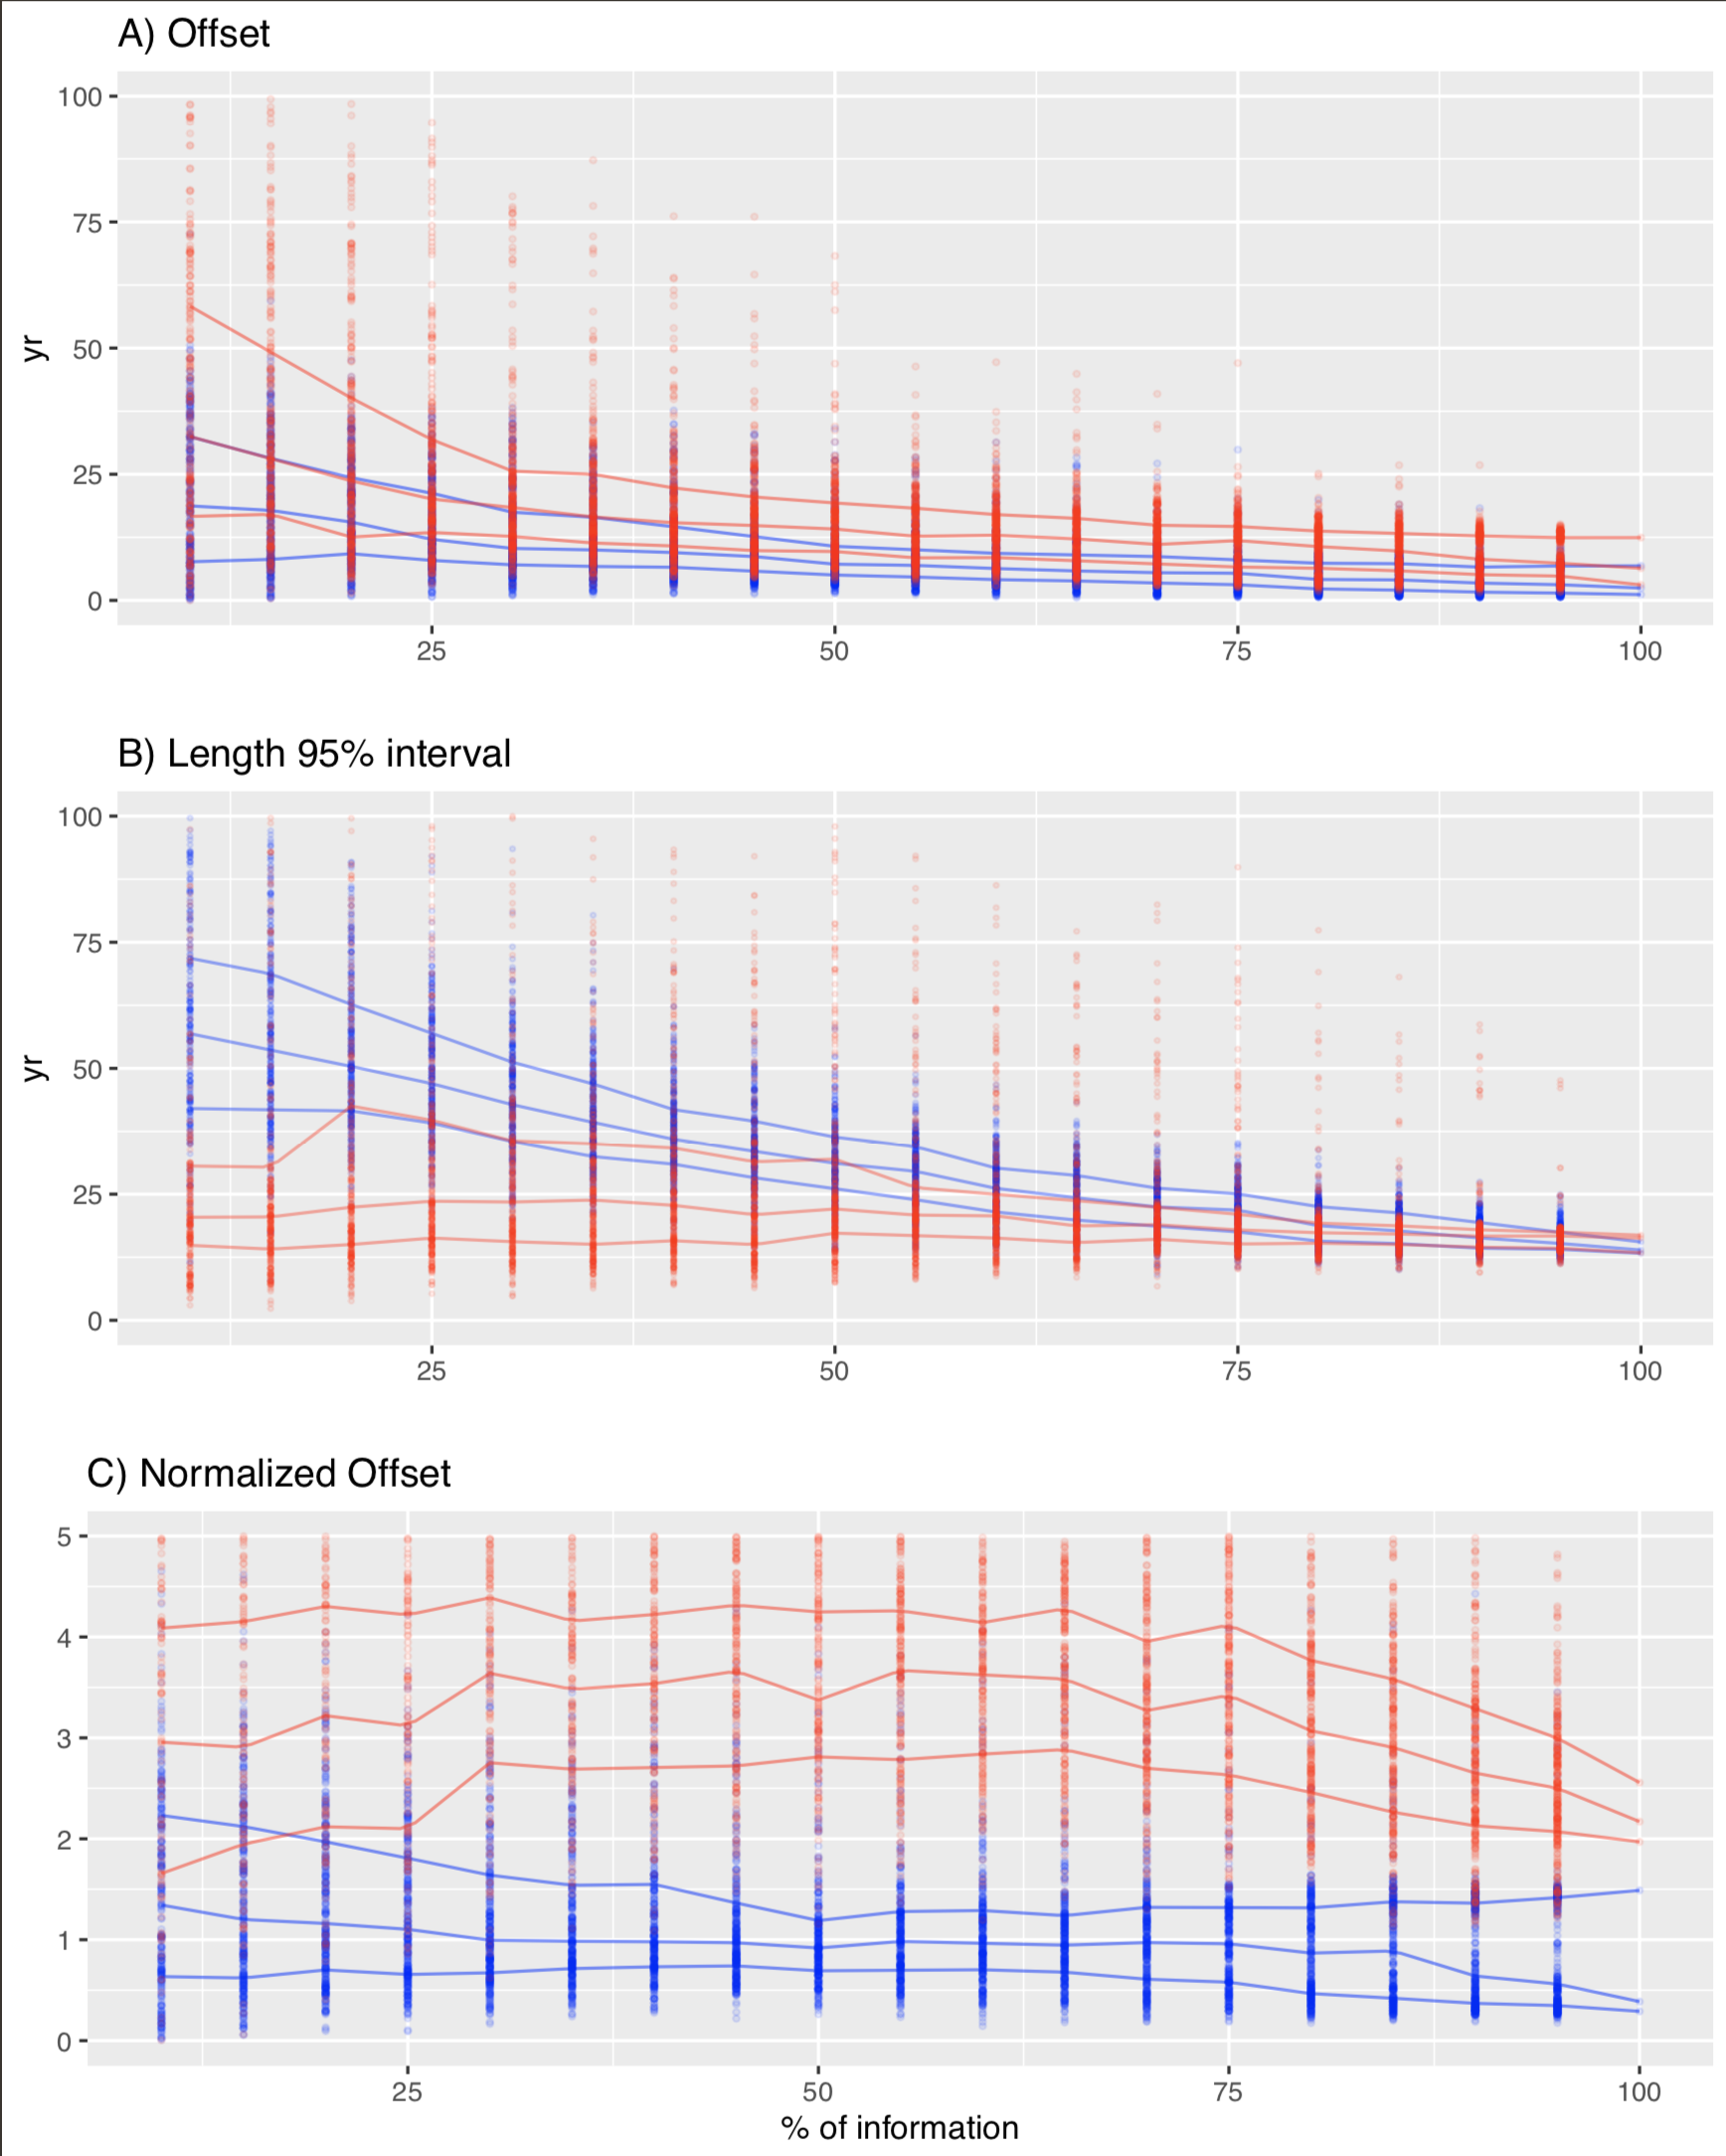
\includegraphics[width=.75\linewidth]{AccPrec.png}
	\caption{Top panel A) shows the offset between the modelled and true age of the CRS (red) and \textit{Plum} (blue). This panel shows how \textit{Plum} provides a small offset in almost every scenario with both models improving their offset as more information is available. Middle panel B) shows the 95\% confidence intervals. It is clear, from this panel, than the uncertainty provided by \textit{Plum} is a lot bigger for low percentage of information and it constantly improves as more data is available, whereas the length of the intervals provided by the CRS appear to stay constant regardless of the available information. Bottom panel C) shows the normalized offsets, presenting the distance between the modelled age and the true age normalized divided by the standard deviation (in the case of \textit{Plum}, the length of the 95\% interval divided by 4). This panel presents a worrying situation where the CRS model's calculated standard deviation (on average) is incapable of of capturing the true age. On the other hand, \textit{Plum}'s credible intervals almost always capture the true age even when little information is available.}
  \label{fig:accpre}
\end{figure}


Figure \ref{fig:accpre} show results similar to those presented by \citet{Blaauw2018}. 
The classical model (CRS) at first appears to provide a similar results (similar offsets) to the Bayesian alternative (\textit{Plum}), but at higher estimated precision (if we only look at the length of the 95\% interval). 
These results can be misleading if we do not consider both the effects of both the offset and length of the interval together. 
To have a more realistic representation of how the models capture the true age-depth models relationship, we should observe the normalized offset. 
This variable shows the degree the average models contain the truth within their uncertainty intervals (normalized to one standard deviation). 
Any model with a normalized offset larger than two (two standard deviations) is incapable of capturing the true ages within its uncertainty intervals.  
This means that, while the CRS estimates smaller uncertainties, it does so at the cost of its accuracy.
It also appears that the length of the 95\% interval and offset are not affected by how much information is provided to the CRS model. 

On the other hand, \textit{Plum} seems to provide increasingly accurate results as more information is added to the model.
This again coincides with the results outlined by \citet{Blaauw2018}. 
When we observe the regular offset (not normalized), we find that textit{Plum} provides a smaller offset in comparison to the CRS model; this in combination with slightly larger modelled uncertainties results in more consistently accurate age-depth models which are capable of capturing the true values within their uncertainty intervals. 
This result supports the claim that \textit{Plum} provides more realistic uncertainties than those of the CRS. 
Another important statistic to take into account is that 87.86\% (4686/5333) of \textit{Plum}'s runs remain within the 2 standard deviations, opposed to 7.48\% (399/5333) for the CRS model. Furthermore, only 0.54\% (29/5333) of the CRS model runs remain under the 1 standard deviation, which is the most commonly reported interval when reporting CRS results.
We can also observe a clear structure in the way that \textit{Plum} increases its accuracy and precision to obtained a better chronology as more information is available, whereas the CRS model does not appears to learn from additional data. 

These results are presented for the overall chronology (the mean offset, interval and normalized offset of the overall chronology). 
In order to evaluate whether certain models are better predicting ages at certain section of the sediment cores, we have to look at the normalized offset of every depth. 


%\begin{figure}
% \centering
%  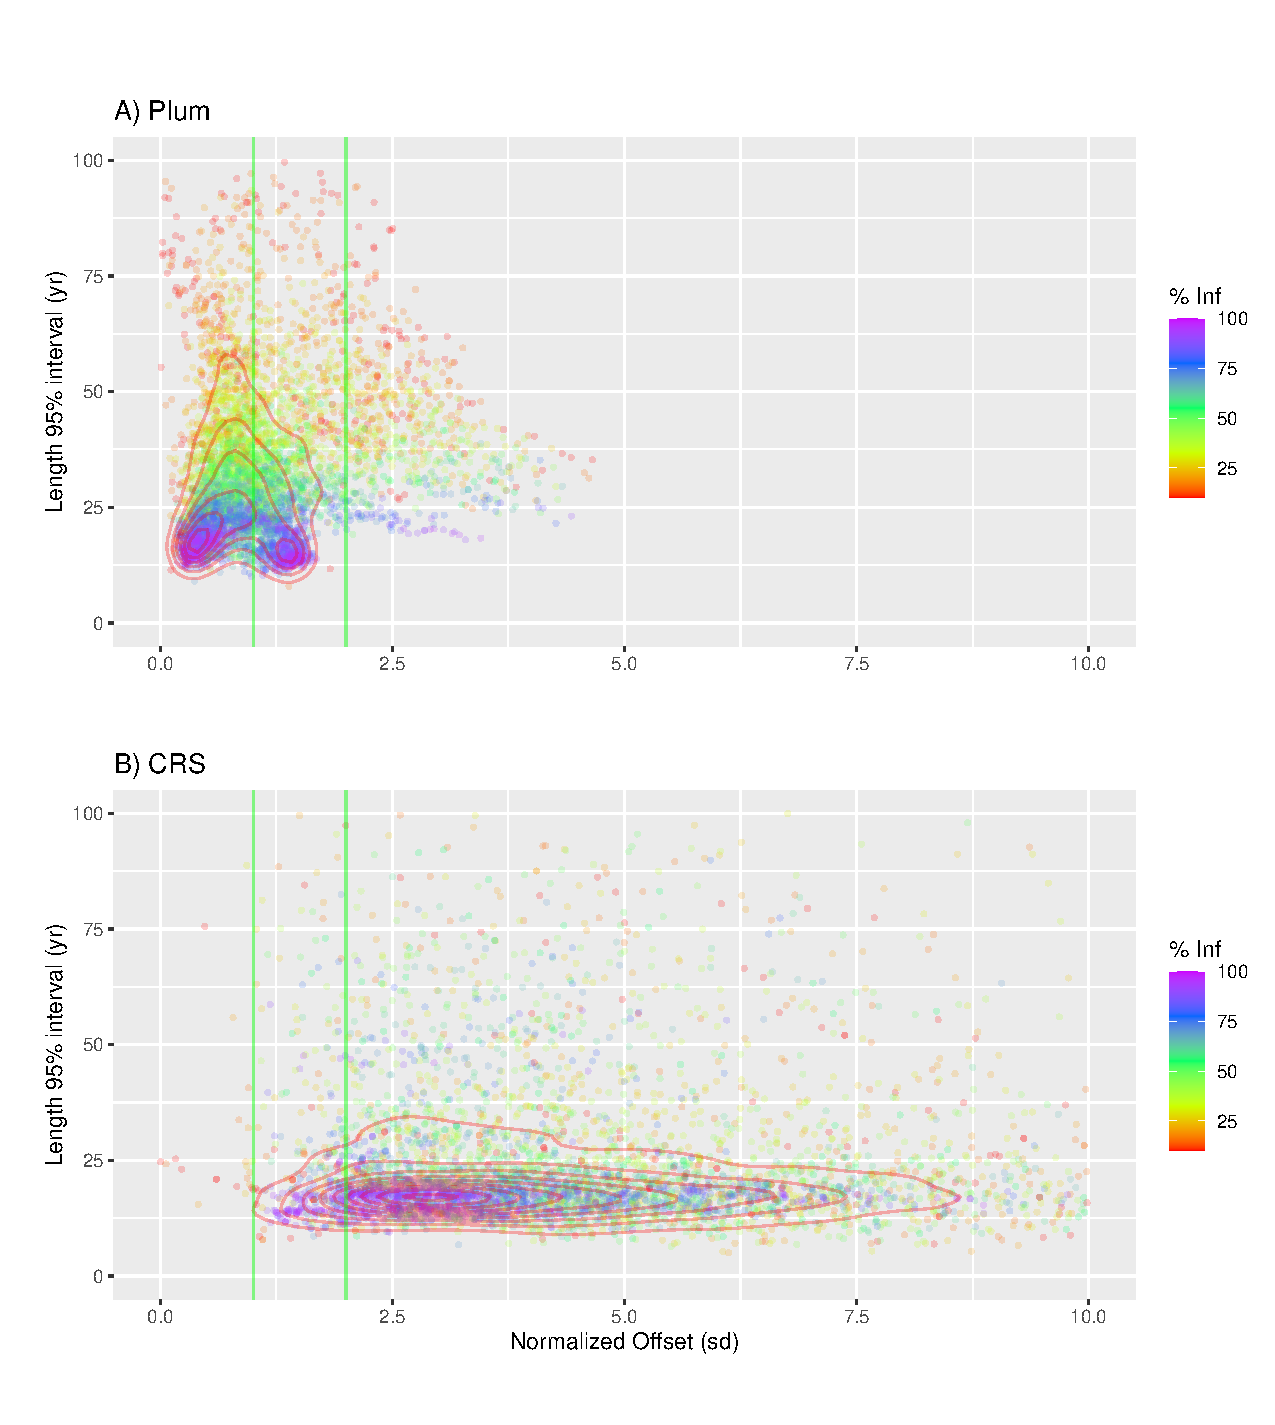
\includegraphics[width=\linewidth]{Maps.pdf}
%	\caption{}
%  \label{fig:maps}
%\end{figure}

%Figure \ref{fig:maps} presents 


\begin{figure}[!]
	\begin{centering}
		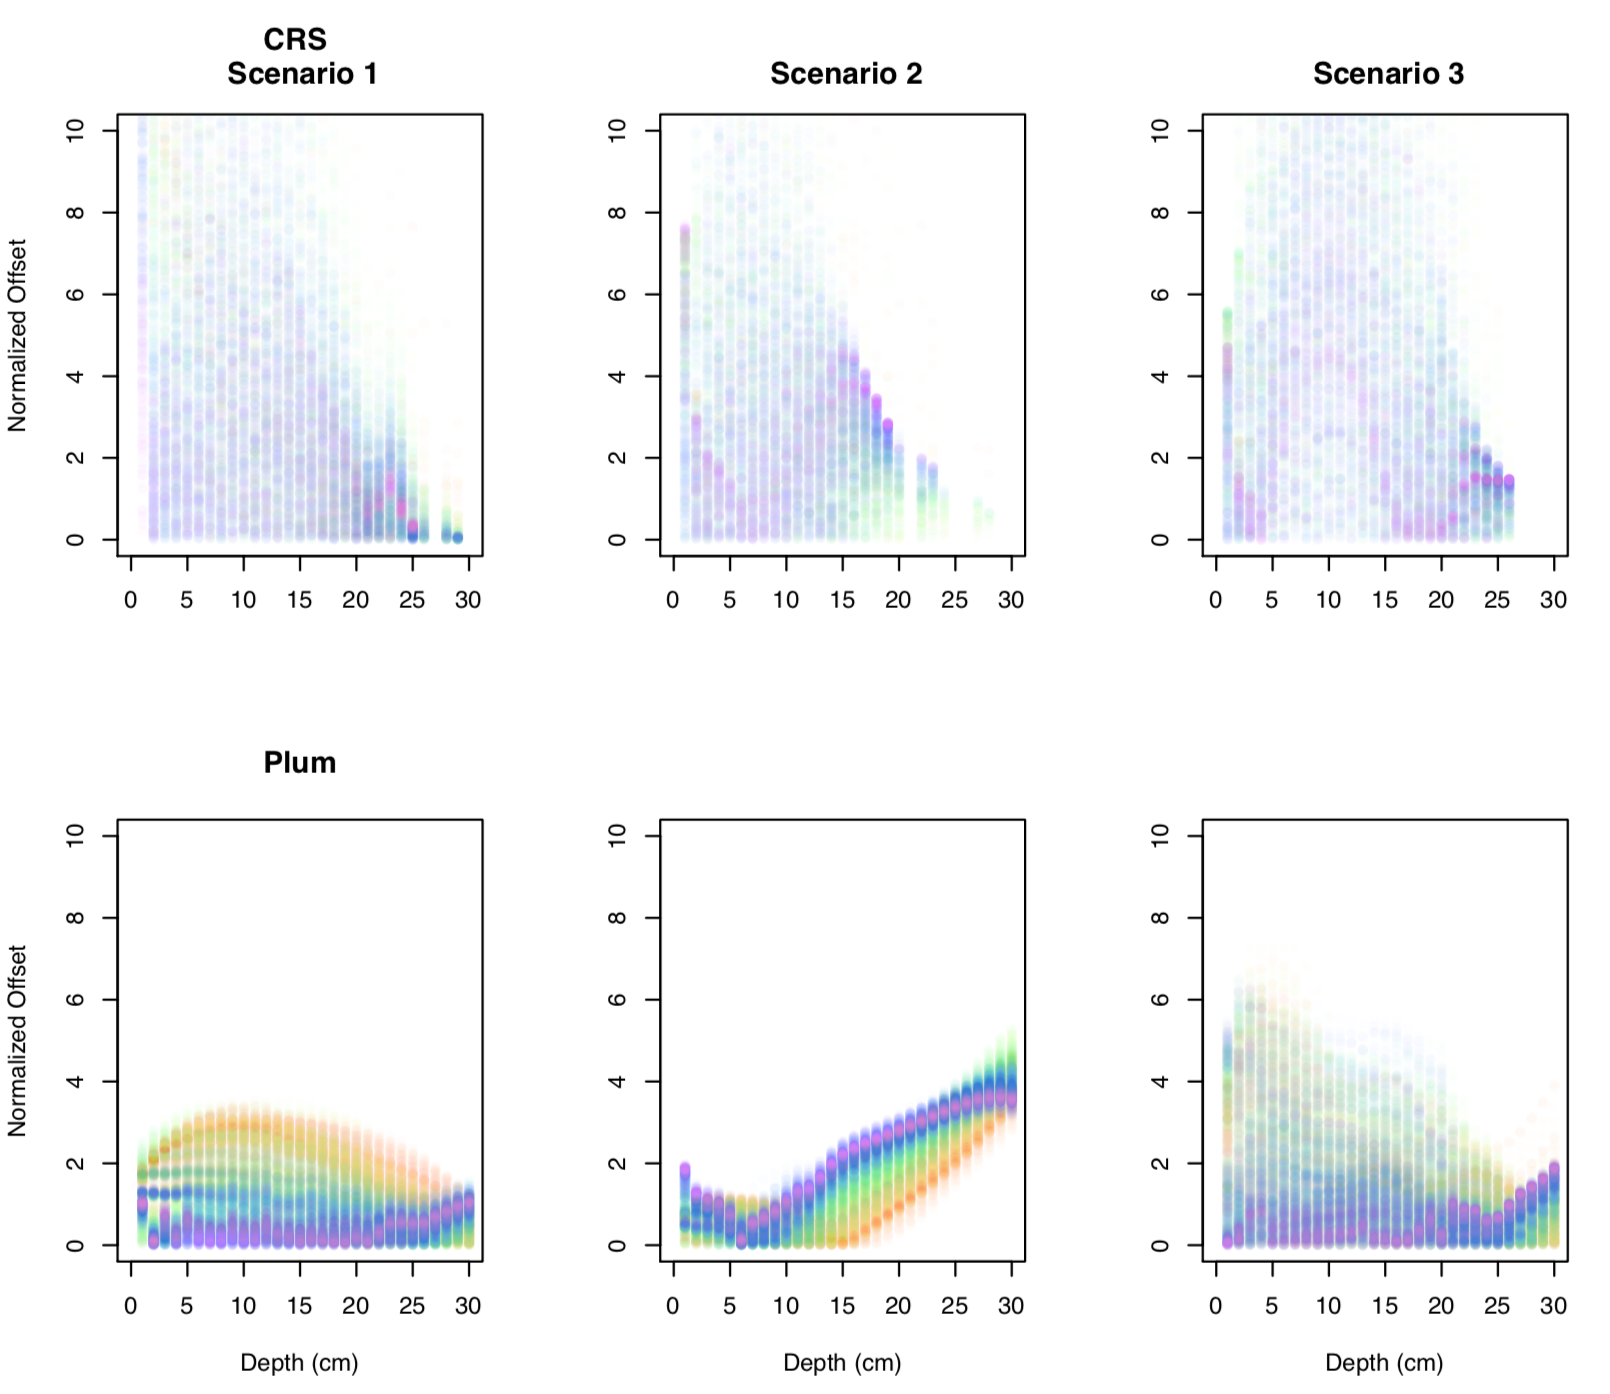
\includegraphics[width=\linewidth]{depths.png}
		\caption{Normalized offset of every sampling sample at every depth for the three simulated scenarios - CRS age estimates at samples depths and \textit{Plum}'s age estimates at 1 cm intervals. Dots go from lowest information percentage samples (few dated depths; red) to high percentage samples (nearly completely dated cores; purple). The CRS's normalized offset shows no structure at any particular depth regardless of the available information. This means that the model can provide a reasonable chronology with low levels of information or a very inaccurate age estimate with high levels of information at any given depth resulting in a distrustful age-depth model. On the other hand, \textit{Plum} demostrares a systematic improvement in its age estimates as more data is available. This results assures that a Bayesian approach would consistently provide more reliable results.     }
		\label{fig:depths}
	\end{centering}
\end{figure}

Figure \ref{fig:depths} shows the normalized accuracy of every simulation according to depth for both models.
\textit{Plum} shows a clear learning structure which depends on the information available to the model.
The information percentage appears to be irrelevant to the accuracy of the CRS model, contrary to the results obtained by \textit{Plum}.
It is important to note that the inaccuracies of the CRS model are not exclusive to any particular sections of the chronology; this is most likely driven by the small uncertainties estimated by the CRS model.See below for a discussion of how \textit{Plum} behaved in sedimentation simulation 2.   


%%%%%%%%%%%%%%%%%%%%%%%%%%%%%%%%%%%%%%%%%%
%%%%%%%%%%%%%%%%%%%%%%%%%%%%%%%%%%%%%%%%%%
\section{Discussion and Conclusions}

These results clearly show the biases associated with the CRS model. 
\citet{Aquino2018} discussed this point and states that the bias is the product of the use of a logarithmic function for the age-depth model. 
It is also evident from these results that the CRS model's uncertainty estimates are not sufficient to capture the true age-depth function. 
This is an important point given the fact that it is common practice among the $^{210}$Pb dating community to report credible intervals to one single deviation, instead of the 95\% confidence intervals, which have become the norm in most other chronological reconstructions.
Other confidence intervals can be calculated for this model \citep{Sanchez-Cabeza2014} but the fact that these intervals are even smaller than the ones obtained by error propagation \citep{Appleby2001} is of concern. 

Previous work on model comparison \citep{Barsanti2020} has shown the problems with the variability of $^{210}$Pb dating results from different users, even when the same or similar models are applied to a single data set.
In our study, user input was reduced to the minimum in an effort to show the potential effects that different percentage of information have on the resulting chronology. 
The results of this experiment showed that the CRS model can provide extremely different results with data originating from the same data set, even while the effect of user input is mitigated. 
Figure \ref{fig:accpre} showed that the CRS model appears not to learn from using more data.
This explains why over the years, many authors have insisted in the use of other dating techniques to validate the chronologies provided by the CRS model \citep{Sanchez-Cabeza2012,Barsanti2020,Aquino2020}, a point which these results also highly encourage.


On the other hand, \textit{Plum} shows a consistently accurate result by capturing the true values within the 95\% credible intervals for most of the simulated sampling strategies. 
It is important to note that one of the big advantages of \textit{Plum} is its increase in accuracy and precision as more data becomes available.
In the case of scenario 2, we observe that \textit{Plum} appears to behaves worse as more data is available, which would be of concern if we did not take into consideration that this sedimentation simulation was extremely unusual in the real world and also if users would not double check the resulting chronologies. 
If more information is available about the core or the sediment, such as $^{210}$Pb influx rates, prior sedimentation rates or independent dating marker, this information can easily be implemented as prior information in \textit{Plum}, and this will result in a much better chronology.
It is also important to note that even when \textit{Plum} performs less well in this specific case, it is providing a much better chronology in upper first 10-15 cm of the core than that of the chaotic CRS age-depth model model.


In conclusion, the use of CRS can only be recommended if users may validate their chronology with external dates as the $^{137}$Cs time markers or other time markers. If not additional information is available for this validation, the use of \textit{Plum}, the Bayesian approach, is still valid, specially if provide it with as as many $^{210}$Pb measurements as possible (at least 60\% of the available information of the core).  Even so, additional dating information may also be formally included in \textit{Plum} to improve the resulting chronology \citep{Aquino2018,Aquino2020}. 


\bibliographystyle{apalike}
\bibliography{bibliography.bib}
\newpage




\section{Supplementary Material}
\label{sec:supp_mat}
Data for each simulation and code used is hosted at: https://github.com/maquinolopez/Paper\_Simulations
\newpage
\begin{table}[h]
	\begin{tabular}{c|cllllll}
		Label    & Depth & Density  & 210Pb & sd(210Pb) & Thickness& 226Ra  & sd(226Ra) \\
		& (cm) &($g/cm^3$) &(Bq/kg)& & (cm) & (Bq/kg)&\\
		\hline 
		Sim01-01 & 1          & 0.10009                         & 63.50103      & 2.85755   & 1              & 23.8045       & 1.125     \\
		Sim01-02 & 2          & 0.10064                         & 80.08738      & 3.60393   & 1              & 23.2924       & 1.125     \\
		Sim01-03 & 3          & 0.10173                         & 98.32806      & 4.42476   & 1              & 23.434        & 1.125     \\
		Sim01-04 & 4          & 0.10334                         & 125.45705     & 5.64557   & 1              & 26.0873       & 1.125     \\
		Sim01-05 & 5          & 0.10547                         & 141.27971     & 6.35759   & 1              & 22.8041       & 1.125     \\
		Sim01-06 & 6          & 0.10809                         & 130.27571     & 5.86241   & 1              & 23.4333       & 1.125     \\
		Sim01-07 & 7          & 0.11116                         & 134.04051     & 6.03182   & 1              & 25.6156       & 1.125     \\
		Sim01-08 & 8          & 0.11466                         & 129.69245     & 5.83616   & 1              & 26.1371       & 1.125     \\
		Sim01-09 & 9          & 0.11855                         & 134.93655     & 6.07214   & 1              & 25.4813       & 1.125     \\
		Sim01-10 & 10         & 0.12278                         & 109.39886     & 4.92295   & 1              & 25.8877       & 1.125     \\
		Sim01-11 & 11         & 0.12731                         & 110.68133     & 4.98066   & 1              & 24.4414       & 1.125     \\
		Sim01-12 & 12         & 0.13209                         & 102.38094     & 4.60714   & 1              & 24.9053       & 1.125     \\
		Sim01-13 & 13         & 0.13706                         & 75.80895      & 3.4114    & 1              & 22.9151       & 1.125     \\
		Sim01-14 & 14         & 0.14218                         & 77.60406      & 3.49218   & 1              & 24.4808       & 1.125     \\
		Sim01-15 & 15         & 0.14738                         & 68.4401       & 3.0798    & 1              & 24.9343       & 1.125     \\
		Sim01-16 & 16         & 0.15262                         & 60.72037      & 2.73242   & 1              & 25.2659       & 1.125     \\
		Sim01-17 & 17         & 0.15782                         & 50.28147      & 2.26267   & 1              & 22.961        & 1.125     \\
		Sim01-18 & 18         & 0.16294                         & 44.24641      & 1.99109   & 1              & 22.9139       & 1.125     \\
		Sim01-19 & 19         & 0.16791                         & 39.85997      & 1.7937    & 1              & 28.3774       & 1.125     \\
		Sim01-20 & 20         & 0.17269                         & 38.40823      & 1.72837   & 1              & 23.5379       & 1.125     \\
		Sim01-21 & 21         & 0.17722                         & 32.75922      & 1.47416   & 1              & 25.4363       & 1.125     \\
		Sim01-22 & 22         & 0.18145                         & 28.02545      & 1.26115   & 1              & 24.8995       & 1.125     \\
		Sim01-23 & 23         & 0.18534                         & 27.8749       & 1.25437   & 1              & 22.6783       & 1.125     \\
		Sim01-24 & 24         & 0.18884                         & 30.74797      & 1.38366   & 1              & 24.8575       & 1.125     \\
		Sim01-25 & 25         & 0.19191                         & 28.36187      & 1.27628   & 1              & 24.8724       & 1.125     \\
		Sim01-26 & 26         & 0.19453                         & 27.24535      & 1.22604   & 1              & 24.3778       & 1.125     \\
		Sim01-27 & 27         & 0.19666                         & 23.59236      & 1.06166   & 1              & 24.7209       & 1.125     \\
		Sim01-28 & 28         & 0.19827                         & 25.74855      & 1.15868   & 1              & 24.6615       & 1.125     \\
		Sim01-29 & 29         & 0.19936                         & 25.05368      & 1.12742   & 1              & 24.7199       & 1.125     \\
		Sim01-30 & 30         & 0.19991                         & 25.0065       & 1.12529   & 1              & 24.4937       & 1.125    
	\end{tabular}
\end{table}


\begin{table}[h]
	\begin{tabular}{c|cllllll}
		Label    & Depth& Density& 210Pb & sd(210Pb) & Thickness & 226Ra & sd(226Ra) \\
				& (cm) &($g/cm^3$) &(Bq/kg)& & (cm) & (Bq/kg)&\\
		\hline 
		Sim02-01 & 1          & 0.1001                          & 909.3928      & 40.9227   & 1              & 8.9761        & 0.45      \\
		Sim02-02 & 2          & 0.1006                          & 683.9989      & 30.7799   & 1              & 10.0607       & 0.45      \\
		Sim02-03 & 3          & 0.1017                          & 453.0503      & 20.3873   & 1              & 9.8701        & 0.45      \\
		Sim02-04 & 4          & 0.1033                          & 310.7897      & 13.9855   & 1              & 10.37         & 0.45      \\
		Sim02-05 & 5          & 0.1055                          & 218.0058      & 9.8103    & 1              & 10.0418       & 0.45      \\
		Sim02-06 & 6          & 0.1081                          & 158.6974      & 7.1414    & 1              & 10.104        & 0.45      \\
		Sim02-07 & 7          & 0.1112                          & 113.9062      & 5.1258    & 1              & 10.2049       & 0.45      \\
		Sim02-08 & 8          & 0.1147                          & 75.5493       & 3.3997    & 1              & 9.334         & 0.45      \\
		Sim02-09 & 9          & 0.1185                          & 56.6252       & 2.5481    & 1              & 10.5145       & 0.45      \\
		Sim02-10 & 10         & 0.1228                          & 44.1595       & 1.9872    & 1              & 9.8677        & 0.45      \\
		Sim02-11 & 11         & 0.1273                          & 34.7448       & 1.5635    & 1              & 9.7694        & 0.45      \\
		Sim02-12 & 12         & 0.1321                          & 25.384        & 1.1423    & 1              & 10.5134       & 0.45      \\
		Sim02-13 & 13         & 0.1371                          & 24.0007       & 1.08      & 1              & 10.4589       & 0.45      \\
		Sim02-14 & 14         & 0.1422                          & 21.3643       & 1         & 1              & 9.9504        & 0.45      \\
		Sim02-15 & 15         & 0.1474                          & 17.7932       & 1         & 1              & 10.5135       & 0.45      \\
		Sim02-16 & 16         & 0.1526                          & 15.0416       & 1         & 1              & 10.3362       & 0.45      \\
		Sim02-17 & 17         & 0.1578                          & 14.2937       & 1         & 1              & 10.5131       & 0.45      \\
		Sim02-18 & 18         & 0.1629                          & 12.3844       & 1         & 1              & 10.368        & 0.45      \\
		Sim02-19 & 19         & 0.1679                          & 12.6023       & 1         & 1              & 10.5297       & 0.45      \\
		Sim02-20 & 20         & 0.1727                          & 11.9329       & 1         & 1              & 10.0924       & 0.45      \\
		Sim02-21 & 21         & 0.1772                          & 9.301         & 1         & 1              & 10.118        & 0.45      \\
		Sim02-22 & 22         & 0.1815                          & 10.7777       & 1         & 1              & 10.249        & 0.45      \\
		Sim02-23 & 23         & 0.1853                          & 12.9491       & 1         & 1              & 10.134        & 0.45      \\
		Sim02-24 & 24         & 0.1888                          & 10.6571       & 1         & 1              & 10.1151       & 0.45      \\
		Sim02-25 & 25         & 0.1919                          & 9.6297        & 1         & 1              & 9.6608        & 0.45      \\
		Sim02-26 & 26         & 0.1945                          & 8.4331        & 1         & 1              & 8.7821        & 0.45      \\
		Sim02-27 & 27         & 0.1967                          & 10.4921       & 1         & 1              & 9.8995        & 0.45      \\
		Sim02-28 & 28         & 0.1983                          & 11.135        & 1         & 1              & 9.2481        & 0.45      \\
		Sim02-29 & 29         & 0.1994                          & 10.109        & 1         & 1              & 10.4398       & 0.45      \\
		Sim02-30 & 30         & 0.1999                          & 9.5404        & 1         & 1              & 10.1114       & 0.45     
	\end{tabular}
\end{table}



\begin{table}[h]
	\begin{tabular}{c|cllllll}
		Label    & Depth & Density & 210Pb & sd(210Pb) & Thickness & 226Ra   & sd(226Ra) \\
						& (cm) &($g/cm^3$) &(Bq/kg)& & (cm) & (Bq/kg)&\\
		\hline 
		Sim03-01 & 1     & 0.1001  & 6384.1354     & 287.2861  & 1         & 15.8007 & 0.675     \\
		Sim03-02 & 2     & 0.1006  & 3550.0809     & 159.7536  & 1         & 14.5245 & 0.675     \\
		Sim03-03 & 3     & 0.1017  & 1954.5702     & 87.9557   & 1         & 15.6527 & 0.675     \\
		Sim03-04 & 4     & 0.1033  & 1183.8917     & 53.2751   & 1         & 14.5175 & 0.675     \\
		Sim03-05 & 5     & 0.1055  & 760.2132      & 34.2096   & 1         & 14.9242 & 0.675     \\
		Sim03-06 & 6     & 0.1081  & 360.2553      & 16.2115   & 1         & 14.801  & 0.675     \\
		Sim03-07 & 7     & 0.1112  & 212.9402      & 9.5823    & 1         & 14.8738 & 0.675     \\
		Sim03-08 & 8     & 0.1147  & 104.2684      & 4.6921    & 1         & 14.9028 & 0.675     \\
		Sim03-09 & 9     & 0.1185  & 44.3849       & 1.9973    & 1         & 15.0768 & 0.675     \\
		Sim03-10 & 10    & 0.1228  & 18.6447       & 1         & 1         & 15.3764 & 0.675     \\
		Sim03-11 & 11    & 0.1273  & 23.2778       & 1.0475    & 1         & 14.6231 & 0.675     \\
		Sim03-12 & 12    & 0.1321  & 53.1587       & 2.3921    & 1         & 15.1629 & 0.675     \\
		Sim03-13 & 13    & 0.1371  & 97.363        & 4.3813    & 1         & 14.3047 & 0.675     \\
		Sim03-14 & 14    & 0.1422  & 116.9788      & 5.264     & 1         & 14.0261 & 0.675     \\
		Sim03-15 & 15    & 0.1474  & 153.2901      & 6.8981    & 1         & 15.9723 & 0.675     \\
		Sim03-16 & 16    & 0.1526  & 151.8496      & 6.8332    & 1         & 14.7579 & 0.675     \\
		Sim03-17 & 17    & 0.1578  & 136.3609      & 6.1362    & 1         & 16.114  & 0.675     \\
		Sim03-18 & 18    & 0.1629  & 107.2736      & 4.8273    & 1         & 15.4595 & 0.675     \\
		Sim03-19 & 19    & 0.1679  & 76.8966       & 3.4603    & 1         & 15.9439 & 0.675     \\
		Sim03-20 & 20    & 0.1727  & 48.9213       & 2.2015    & 1         & 14.6235 & 0.675     \\
		Sim03-21 & 21    & 0.1772  & 40.4439       & 1.82      & 1         & 14.6716 & 0.675     \\
		Sim03-22 & 22    & 0.1815  & 26.5638       & 1.1954    & 1         & 16.2541 & 0.675     \\
		Sim03-23 & 23    & 0.1853  & 21.714        & 1         & 1         & 14.4826 & 0.675     \\
		Sim03-24 & 24    & 0.1888  & 17.6428       & 1         & 1         & 15.5109 & 0.675     \\
		Sim03-25 & 25    & 0.1919  & 17.3533       & 1         & 1         & 13.6898 & 0.675     \\
		Sim03-26 & 26    & 0.1945  & 17.4211       & 1         & 1         & 14.4684 & 0.675     \\
		Sim03-27 & 27    & 0.1967  & 16.4246       & 1         & 1         & 15.3889 & 0.675     \\
		Sim03-28 & 28    & 0.1983  & 12.4828       & 1         & 1         & 15.0698 & 0.675     \\
		Sim03-29 & 29    & 0.1994  & 13.5514       & 1         & 1         & 15.2346 & 0.675     \\
		Sim03-30 & 30    & 0.1999  & 14.3145       & 1         & 1         & 14.7846 & 0.675    
	\end{tabular}
\end{table}



\end{document}
